\documentclass[a4paper, 14pt]{extarticle}

% file's preambule

% Если вы работаете не в XeLaTeX, то сами разбирайтесь =)

% connect packages
%%%%%%%%%%%%%%%%%%%%%%%%%%%%%%%%%%%%%%%%%%%%%%%%%%%%%%%%%%%%%%%%%%%%%%
%\usepackage[T2A]{fontenc}                   %!? закрепляет внутреннюю кодировку LaTeX
%\usepackage[utf8]{inputenc}                 %!  закрепляет кодировку utf8
\usepackage{fontspec}                        % Шрифты
\usepackage{indentfirst}                    %   добавить indent перед первым параграфом
\setlength{\parindent}{1.27cm}
\usepackage{polyglossia}                     % Русский язык
\setdefaultlanguage{russian}
\setmainfont[Ligatures=TeX]{Times New Roman}
\newfontfamily\cyrillicfont{Times New Roman}[Script=Cyrillic]
%\usepackage[english,russian]{babel}         %!  подключает русский и английский
\usepackage{amsmath}                        %!  |
\usepackage{amssymb,textcomp, esvect,esint} %!  |важно для формул 
\usepackage{geometry}                       %!  отступ от граней
\geometry{verbose,a4paper,tmargin=2cm,bmargin=2cm,lmargin=3cm,rmargin=1cm}
\usepackage{amsfonts}                       %!  математические шрифты
\usepackage{amsthm}                         %!  newtheorem и их сквозная нумерация
\usepackage{graphicx}                       %?  графическое изменение текста
\usepackage{soulutf8}% Поддержка переносоустойчивых подчёркиваний и зачёркиваний
\usepackage{enumitem}                       %!  задание макета перечня.
%\usepackage[unicode, pdftex]{hyperref}      %!  оглавление для панели навигации по PDF-документу + гиперссылки
\usepackage{setspace}                       % Межстроковые интервалы
\onehalfspacing
\usepackage{booktabs}                       %!  добавляет книжные линии в таблицы
%\usepackage{hypcap}                         %?  адресация на картинку, а не на подпись к ней
\usepackage{abraces}                        %?  фигурные скобки сверху или снизу текста
\usepackage{caption}                        %-  позволяет корректировать caption 
\DeclareCaptionLabelSeparator{dash}{ - }
\captionsetup[table]{labelformat=simple, labelsep=dash, justification=raggedleft,
singlelinecheck=off}
\captionsetup[figure]{labelformat=simple, labelsep=dash}
\usepackage{multirow}                       %   объединение ячеек в таблицах
\usepackage{longtable}
\usepackage{pifont}                         %!  нужен для крестика
\usepackage{cancel}                         %!  аутентичное перечеркивание текста
\usepackage{ulem}                           %!  перечеркивание текста
\usepackage{tikz}                           %!  высокоуровневые рисунки (кружочек)
\usepackage{titling}                        %-  автоматическое заглавие 
\usepackage{titlesec}  % нормальные заголовки секций
\titleformat{\section}
{\normalfont\large\bfseries\filcenter}{}{1em}{}
\titleformat{\subsection}
  {\normalfont\normalsize\bfseries}{\thesubsection.}{5pt}{}
\titleformat{\subsubsection}
  {\normalfont\normalsize\bfseries}{\thesubsubsection.}{5pt}{}
\titleformat{\paragraph}
  {\normalfont\normalsize\bfseries}{\theparagraph}{5pt}{}

\usepackage{ragged2e} % Для выравнивания текста по ширине
\justifying

%\renewcommand{\thesubsubsection}{\alph{subsubsection}}
\usepackage{blindtext}                      %-  слепой текст
\usepackage{fancyhdr}                       %   добавить верхний и нижний колонтитул
\usepackage{mathptmx}

\usepackage{import}                         %|
\usepackage{xifthen}                        %|
\usepackage{pdfpages}                       %|
%\usepackage{transparent}                    %| вставка ink figures
\usepackage{rotating}
\usepackage{array} % Картиночки в таблицы
%%%%%%%% Алгоритмы
\usepackage{float}
\usepackage{algorithm}
\usepackage{algpseudocode}
%%%%%%%%%%%%%%%

\usepackage{listings} % Для языков программирования 
\usepackage{xcolor}
\lstset {
    language=C++,
    backgroundcolor=\color{black!5}, % set backgroundcolor
    basicstyle=\footnotesize,% basic font setting
}

\usepackage{lmodern}

\colorlet{comment}{green!50!black}
\colorlet{cppcomment}{teal}
\colorlet{symb}{blue!50!black}
\colorlet{number}{violet}

\newcommand*{\textcolorsymb}{\textcolor{symb}}

\definecolor{backcolour}{rgb}{0.95,0.95,0.92}
\definecolor{black_red}{rgb}{0.54, 0, 0}

\lstdefinestyle{cpp}{%
  language=C++,
  columns=flexible,
  basewidth=.5em,  
  tabsize=2,
  basicstyle=\footnotesize,
  backgroundcolor=\color{backcolour},
  showspaces=false,
  showstringspaces=false,
  commentstyle={\itshape\color{comment}\let\textcolorsymb\relax},
  keywordstyle=\bfseries\color{black_red},
  morecomment={[l][\itshape\color{cppcomment}\let\textcolorsymb\relax]//},
  literate=%
    {\{}{\textcolorsymb{\{}}1
    {\}}{\textcolorsymb{\}}}1
    {(}{\textcolorsymb{(}}1
    {)}{\textcolorsymb{)}}1
    {;}{\textcolorsymb{;}}1
    {=}{\textcolorsymb{=}}1
    {<}{\textcolorsymb{<}}1
    {>}{\textcolorsymb{>}}1
    {!}{\textcolorsymb{!}}1
    {\&}{\textcolorsymb{\&}}1 
    {|}{\textcolorsymb{|}}1
    {?}{\textcolorsymb{?}}1
    {:}{\textcolorsymb{:}}1
    {+}{\textcolorsymb{+}}1
    {-}{\textcolorsymb{-}}1
    {,}{\textcolorsymb{,}}1
    {\%}{\textcolorsymb{\%}}1
    {\^}{\textcolorsymb{\textasciicircum}}1
    {~}{\textcolorsymb{\textasciitilde}}1
    %% {/}{\textcolorsymb{/}}1
    %% {*}{\textcolorsymb{*}}1
    % 2 (optionally)
    {==}{\textcolorsymb{==}}2
    {>=}{\textcolorsymb{=>}}2
    {<=}{\textcolorsymb{<=}}2
    {!=}{\textcolorsymb{!=}}2
    {+=}{\textcolorsymb{+=}}2
    {-=}{\textcolorsymb{-=}}2
    {*=}{\textcolorsymb{*=}}2
    {/=}{\textcolorsymb{/=}}2
    {\%=}{\textcolorsymb{\%=}}2
    {\&\&}{\textcolorsymb{\&\&}}2
    {||}{\textcolorsymb{||}}2
    {++}{\textcolorsymb{++}}2
    {--}{\textcolorsymb{--}}2
    {>>}{\textcolorsymb{>\kern0pt>}}2
    {<<}{\textcolorsymb{<\kern0pt<}}2
    {::}{\textcolorsymb{::}}2
    % 3 (optionally)
    {>>=}{\textcolorsymb{>\kern0pt>=}}3
    {<<=}{\textcolorsymb{<\kern0pt<=}}3
    % Remove byte order mark
    {^^ef^^bb^^bf}{}0
}
\lstnewenvironment{cpp}{\lstset{style=cpp}}{}
\lstset{style=cpp}
  


%%%%%%%%%%%%%%%%%%%%%%%%%%%%%%%%%%%%%%%%%%%%%%%%%%%%%%%%%%%%%%%%%%%%%%


%%%%%%%%%%%%%%%%%% ВСТАВКА РИСУНКО ИЗ INKSCAPE %%%%%%%%%%%%%%%%%%%%%%%
\newcommand{\incfig}[1]{%
    \def\svgwidth{\columnwidth}
    \import{./figures/}{#1.pdf_tex}
}

%%%%%%%%%%%%%%%%%%%%%%%%%%%%%%%%%%%%%%%%%%%%%%%%%%%%%%%%%%%%%%%%%%%%%%


\newenvironment{itemize*}
{
    \begin{itemize}
        \setlength{\itemsep}{1pt}
        \setlength{\parskip}{1pt}}
    {\end{itemize}
}

\newenvironment{enumerate*}
{
    \begin{enumerate}
        \setlength{\itemsep}{1pt}
        \setlength{\parskip}{1pt}}
    {\end{enumerate}
}

%%%%%%%%%%%%%%%%%%%%%%%%%%%%%%%%%%%%%%%%%%%%%%%%%%%%%%%%%%%%%%%%%%%%%%


\begin{document}

\includepdf{titul_fourth}
\newpage
\tableofcontents
\newpage
\section{Задание 1. Определение эффективного алгоритма в среднем случае}
\noindent 2 Вариант.
\subsection{Сортировка простого обмена с условием Айверсона}
\paragraph{Постановка задачи}
Разработать алгоритм сортировки простого обмена (пузырька) с условием
Айверсона, провести анализ вычислительной и емкостной сложности алгоритма
на массивах, заполненных случайно.
\paragraph{Описание алгоритма сортировки}
При переборе массива попарно сравниваются соседние элементы. Если
порядок их следования не соответствует заданному критерию
упорядоченности, то элементы меняются местами. В результате одного такого
просмотра при сортировке по возрастанию элемент с самым большим
значением ключа переместится («всплывет») на последнее место массива. При
следующем проходе на свое место «всплывет» второй по величине элемент и
т.д. Отсутствие перестановок на какой-либо итерации означает
упорядоченность массива (условие Айверсона).
\newpage
\paragraph{Алгоритм сортировки}
\begin{figure}[htpb]
  \centering
  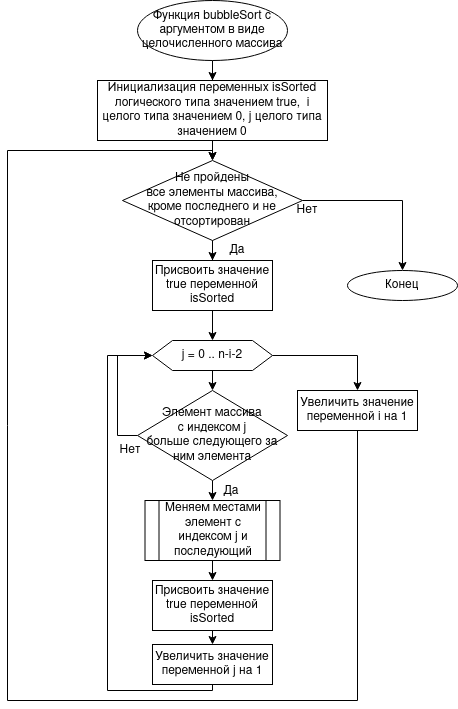
\includegraphics[width=0.7\textwidth]{pictures/first_sort_flowchart.png}
  \caption{Блок-схема сортировки пузырьком с условием Айверсона}
  \label{fig:first_sort_flow}
\end{figure}
\newpage
\paragraph{Оценка функции роста скорости выполнения алгоритма сортировки}
Определим теоретическую сложность алгоритма при помощи таблицы
операторов.

\begin{table}[htpb]
  \centering
  \caption{Подсчет количества операторов в алгоритме сортировки простого обмена}
  \label{tab:first_sort_speed}
  \begin{tabular}{|c|c|c|c|}
    \hline
    \parbox[m]{2cm}{\centering Номер \\ оператора}
    & Оператор
    & \parbox[m]{2cm}{\centering Время выполнения \\ одного оператора}
    & \parbox[m]{2cm}{\centering Кол-во выполнений \\ оператора в строке}
    \\ \hline
    1 & bool isSorted = false; & C1 & 1 раз
    \\ \hline
    2 & \parbox[m]{4cm}{\centering for (int i = 0;\\ !isSorted \&\& i < n-1; ++i) \{ }
      & C2 & n раз
    \\ \hline
      3 & isSorted = true; & C3 & n-1 раз
      \\ \hline
      4 &\parbox[m]{4cm}{\centering for (int j = 0;\\ j < n - i - 1;
         ++j) \{ } & C4 & n(n-1) раз
    \\ \hline
        5 & if (v[j] > v[j+1]) \{  & C5 & n(n-1) - 1 раз
    \\ \hline
    6 & std::swap(v[j], v[j+1]); & C6 & n(n-1) - 1 раз
    \\ \hline
7 & isSorted = false;\}\}\} & C7 & n(n-1) - 1 раз
\\ \hline
  \end{tabular}
\end{table}

Из таблицы \ref{tab:first_sort_speed} получим функцию роста выполнения алгоритма
сортировки простого обмена. Пусть $T(n)$ - время выполнения алгоритма, зависящее
от  $n$. Тогда
\[
  \begin{split}
  T(n) = C_1 + C_2\cdot n + C_3\cdot (n-1) + C_4\cdot (n^2-n) \\
  + C_5\cdot (n^2-n-1) + C_6\cdot (n^2-n-1) + C_7\cdot (n^2-n-1)
  \end{split}
\]

После упрощения получаем
\[
  \begin{split}
  T(n) = C_1 + C_2\cdot n + C_3 \cdot n - C_3 + C_4\cdot n^2
  - C_4\cdot n \\ + C_5\cdot n^2 - C_5\cdot n - C_5
  + C_6\cdot n^2 - C_6\cdot n - C_6\\ + C_7\cdot n^2 - C_7\cdot n - C_7 
  \end{split}
.\]
Подведя подобные, получаем
\[
  T(n) = An^2+Bn+C
.\]
Оставляя справа только доминирующую функцию, получаем порядок роста $T(n)
= O(n^2)$, где  $n$ - размер массива.

\paragraph{Емкостная сложность сортировки}
Емкостная сложность алгоритма порядка $O(n)$ т.к. используется
только исходный массив размера  $n$.

\paragraph{Код функции сортировки}
\begin{figure}[htpb]
  \centering
  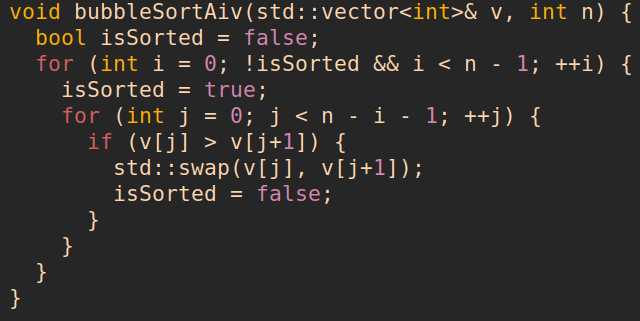
\includegraphics[width=0.7\textwidth]{pictures/first_sort_code.png}
  \caption{Код сортировки пузырьком}
  \label{fig:first_sort_code}
\end{figure}
\paragraph{Тестирование функции сортировки}
\begin{figure}[htpb]
  \centering
  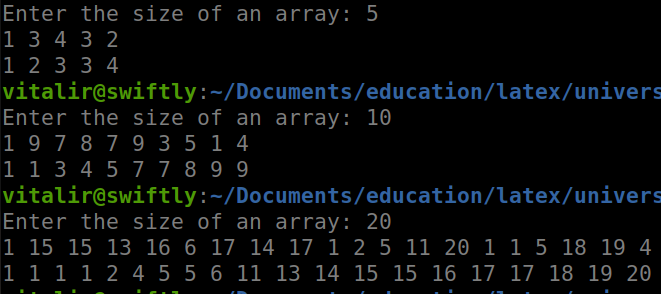
\includegraphics[width=0.7\textwidth]{pictures/first_sort_test.png}
  \caption{Результаты тестирования на работоспособность сортировки пузырьком}
  \label{fig:first_sort_test}
\end{figure}
\newpage
\paragraph{Сводная таблица тестирования}
\begin{figure}[htpb]
  \centering
  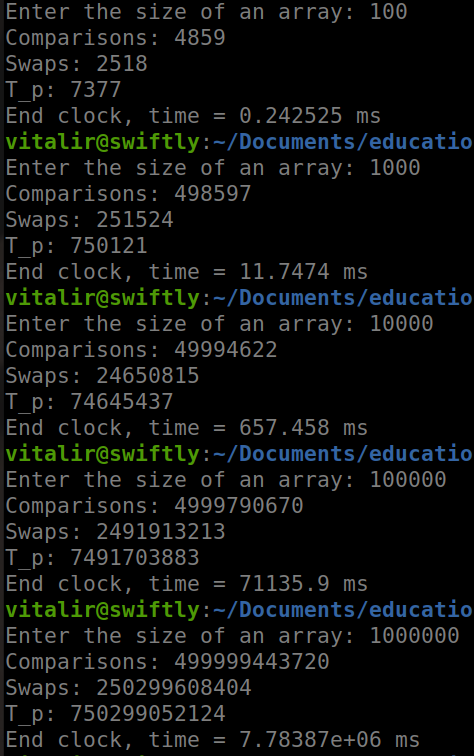
\includegraphics[width=0.7\textwidth]{pictures/first_sort_speed_gen.png}
  \caption{Результаты тестирования сортировки пузырьком}
  \label{fig:first_sort_speed_gen}
\end{figure}
\begin{table}[htpb]
  \centering
  \caption{Сводная таблица тестирования сортировки пузырьком}
  \label{tab:first_sort_test_general}
  \begin{tabular}{|c|c|c|c|}
    \hline
    n & $T(n)$ & $T_\textup Т=f(C+M)$ &
    $T_\textup п=C_\textup ф+M_\textup ф$
    \\ \hline
    100
    & 0.242525 мс
    & \multirow{5}*{\centering $O(n^2)$}
    & 7377
    \\ \cline{1-2}\cline{4-4}
    1000
    & 11.7474 мс
    &
    & 750121
    \\ \cline{1-2}\cline{4-4}
    10000
    & 657.458 мс
    &
    & 74645458
    \\ \cline{1-2}\cline{4-4}
    100000
    & 71135.9 мс
    &
    & 7491703883
    \\ \cline{1-2}\cline{4-4}
    1000000
    & 7783870 мс
    &
    & 750299052124
    \\ \hline
  \end{tabular}
\end{table}
\newpage
Для тестирования был создан класс для подсчета времени TimeCounter;
также была создана версия функции сортировки со встроенной отладкой.
(рисунки \ref{fig:time_counter_code} и \ref{fig:first_sort_log}).
\begin{figure}[htpb]
  \centering
  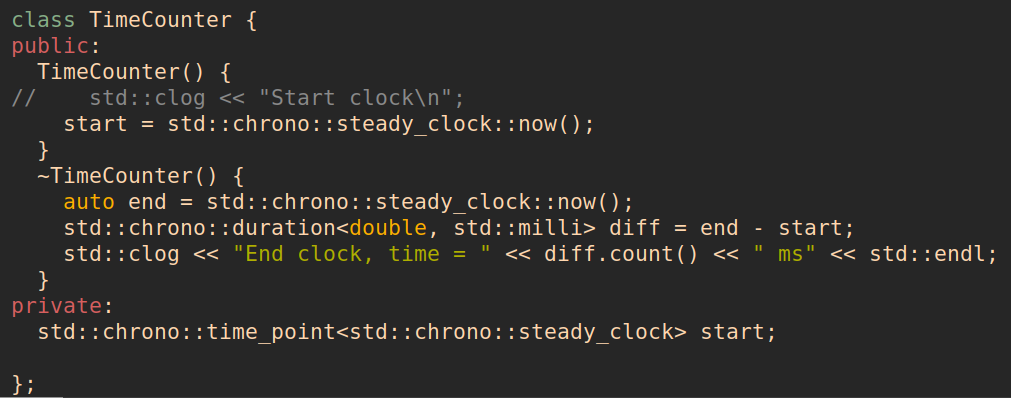
\includegraphics[width=0.8\textwidth]{pictures/time_counter_code.png}
  \caption{Класс TimeCounter}
  \label{fig:time_counter_code}
\end{figure}
\begin{figure}[htpb]
  \centering
  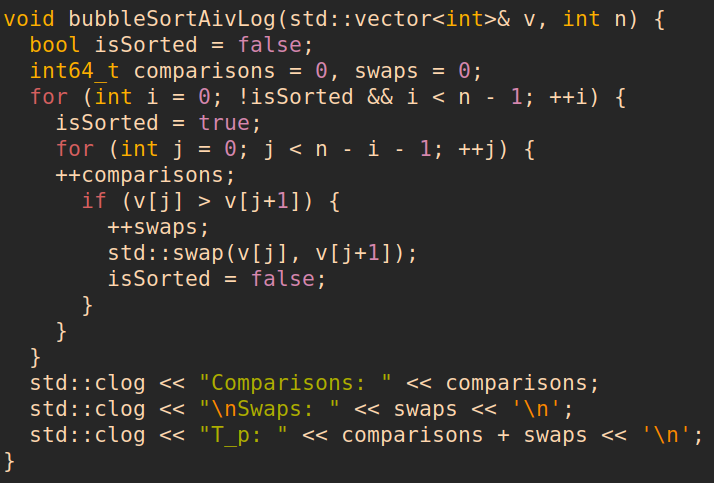
\includegraphics[width=0.7\textwidth]{pictures/first_sort_log.png}
  \caption{Функция bubbleSortAivLog}
  \label{fig:first_sort_log}
\end{figure}
\newpage
\subsection{Шейкерная сортировка}
\paragraph{Постановка задачи}
Разработать алгоритм шейкерной сортировки (двосторонний пузырек),
провести анализ вычислительной и емкостной сложности алгоритма
на массивах, заполненных случайно.
\paragraph{Описание сортировки}
Является улучшенной версией сортировки пузырьком. На первом проходе мы задвигаем
максимальный элемент в конец массива, потом же идем в обратном направлении
и двигаем минимум в начало. Отсортированные крайние области массива увеличиваются
после каждой итерации.
\newpage
\paragraph{Алгоритм сортировки}
\begin{figure}[htpb]
  \centering
  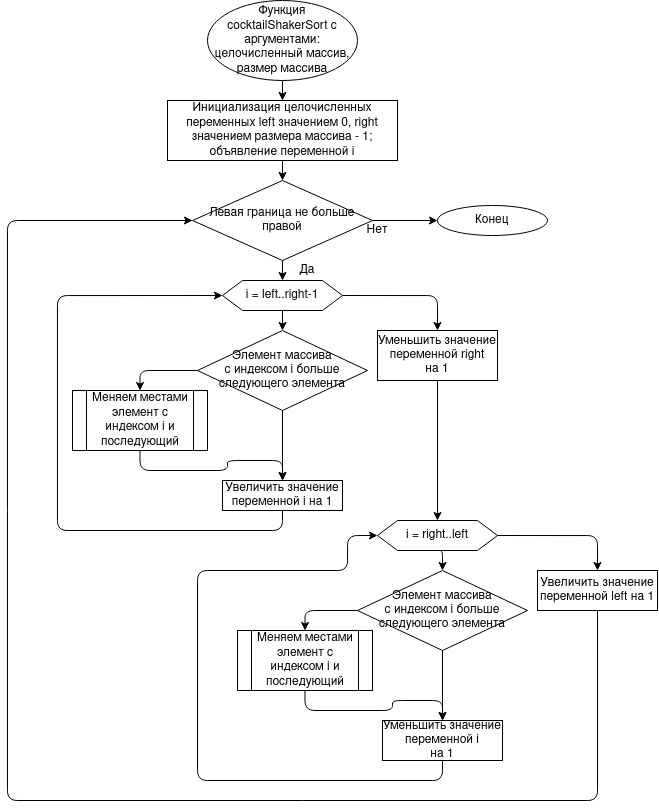
\includegraphics[width=0.8\textwidth]{pictures/second_sort_flowchart.png}
  \caption{Блок-схема шейкерной сортировки}
  \label{fig:second_sort_flow}
\end{figure}
\paragraph{Оценка функции роста скорости выполнения алгоритма сортировки}
Определим теоретическую сложность алгоритма при помощи таблицы
операторов.

\begin{table}[htpb]
  \centering
  \caption{Подсчет количества операторов в алгоритме шейкерной сортировки}
  \label{tab:second_sort_speed}
  \begin{tabular}{|c|c|c|c|}
    \hline
    \parbox[m]{2cm}{\centering Номер \\ оператора}
    & Оператор
    & \parbox[m]{2cm}{\centering Время выполнения \\ одного оператора}
    & \parbox[m]{2cm}{\centering Кол-во выполнений \\ оператора в строке}
    \\ \hline
    1 & \parbox[m]{4cm}{\centering int left = 0; int right = n - 1;}
 & C1 & 1 раз
    \\ \hline
    2 & while (left $\leq$  right)
      & C2 & n раз
    \\ \hline
    3 & \parbox[m]{4cm}{\centering for (int i = left;\\ i < right; ++i) \{ }
      & C3 & n(n-1) раз
      \\ \hline
      4 & if (v[i] > v[i+1]) \{ & C4 & n(n-1)-1 раз
    \\ \hline
    5 & std::swap(v[i], v[i+1])\}\} & C5 & n(n-1)-1 раз
    \\ \hline
    6 & --right; & C6 & n-1 раз
    \\ \hline
    7 & \parbox[m]{4cm}{\centering for (int i = right-1;\\ i $\geq$ left; --i) \{ }
      & C7 & n(n-1) раз
      \\ \hline
      8 & if (v[i] > v[i+1]) \{ & C8 & n(n-1)-1 раз
    \\ \hline
    9 & std::swap(v[i], v[i+1])\}\} & C5 & n(n-1)-1 раз
    \\ \hline
10 & ++left;\} & C10  &  n-1 раз
    \\ \hline
  \end{tabular}
\end{table}

\newpage
Из таблицы \ref{tab:second_sort_speed} получим функцию роста выполнения алгоритма
сортировки простого обмена. Пусть $T(n)$ - время выполнения алгоритма, зависящее
от  $n$. Тогда

\[
  \begin{split}
  T(n) = C_1 + C_2\cdot n + C_3\cdot (n^2-n) + C_4\cdot (n^2-n-1)
  \\ + C_5\cdot (n^2-n-1) + C_6\cdot (n-1) + C_7\cdot (n^2-n)
  \\ + C_8\cdot (n^2-n-1) + C_9\cdot (n^2-n-1) + C_{10}\cdot (n-1) 
  \end{split}
.\]

После упрощения и подведя подобные получаем
\[
  T(n) = An^2+Bn+C
.\]
Оставляя справа только доминирующую функцию, получаем порядок роста
$T(n) = O(n^2)$, где  $n$ - размер массива.

\paragraph{Емкостная сложность сортировки}
Емкостная сложность алгоритма порядка $O(n)$ т.к. используется
только исходный массив размера  $n$.
\paragraph{Код функции сортировки}
\begin{figure}[htpb]
  \centering
  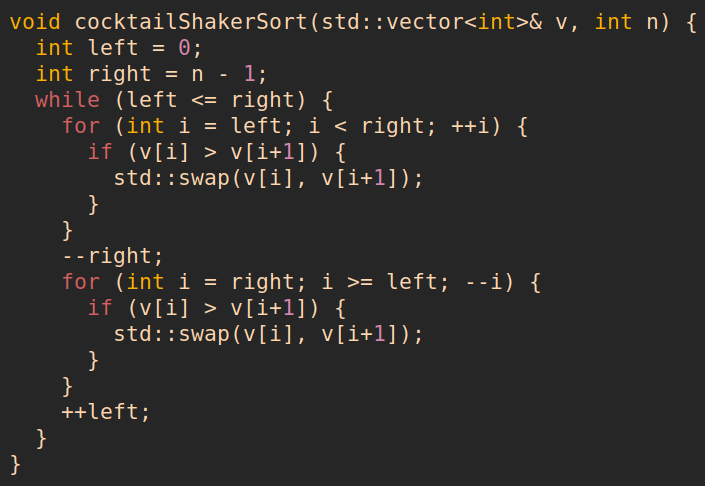
\includegraphics[width=0.7\textwidth]{pictures/second_sort_code.png}
  \caption{Код шейкерной сортировки}
  \label{fig:second_sort_code}
\end{figure}
\paragraph{Тестирование функции сортировки}
\begin{figure}[htpb]
  \centering
  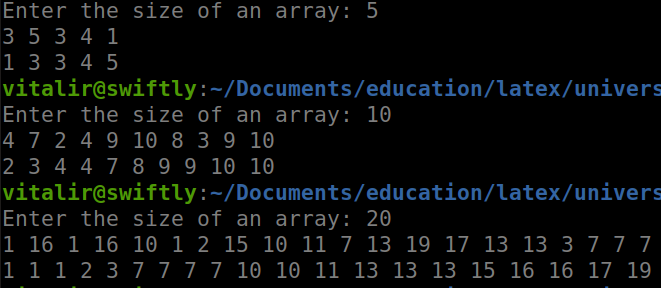
\includegraphics[width=0.7\textwidth]{pictures/second_sort_test.png}
  \caption{Результаты тестирования на работоспособность шейкерной сортировки}
  \label{fig:second_sort_test}
\end{figure}
\newpage
\paragraph{Сводная таблица тестирования}
\begin{figure}[htpb]
  \centering
  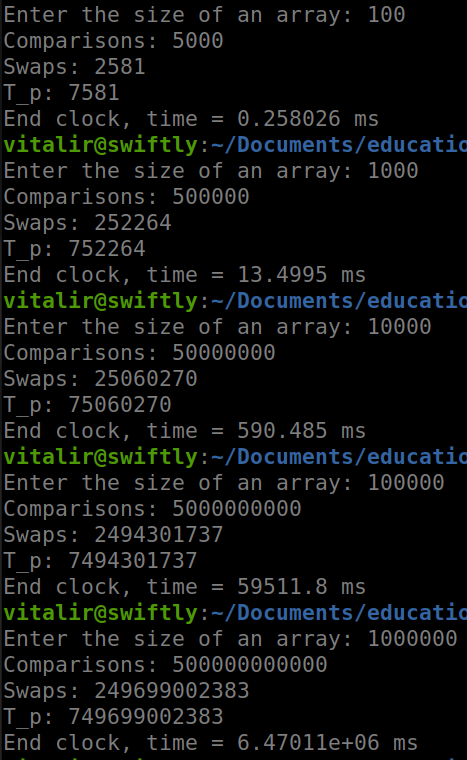
\includegraphics[width=0.47\textwidth]{pictures/second_sort_speed_gen.png}
  \caption{Результаты тестирования шейкерной сортировки}
  \label{fig:second_sort_speed_gen}
\end{figure}
\begin{table}[htpb]
  \centering
  \caption{Сводная таблица тестирования шейкерной сортировки}
  \label{tab:second_sort_test_general}
  \begin{tabular}{|c|c|c|c|}
    \hline
    n & $T(n)$ & $T_\textup Т=f(C+M)$ &
    $T_\textup п=C_\textup ф+M_\textup ф$
    \\ \hline
    100
    & 0.258026 мс
    & \multirow{5}*{\centering $O(n^2)$}
    & 7581
    \\ \cline{1-2}\cline{4-4}
    1000
    & 13.4995 мс
    &
    & 752264
    \\ \cline{1-2}\cline{4-4}
    10000
    & 590.485 мс
    &
    & 75060270
    \\ \cline{1-2}\cline{4-4}
    100000
    & 59511.8 мс
    &
    & 7494301737
    \\ \cline{1-2}\cline{4-4}
    1000000
    & 6470110 мс
    &
    & 749699002383
    \\ \hline
  \end{tabular}
\end{table}

Для тестирования был использован класс для подсчета времени TimeCounter;
также была создана версия функции сортировки со встроенной отладкой.
(рисунки \ref{fig:time_counter_code} и \ref{fig:second_sort_log}).
\begin{figure}[htpb]
  \centering
  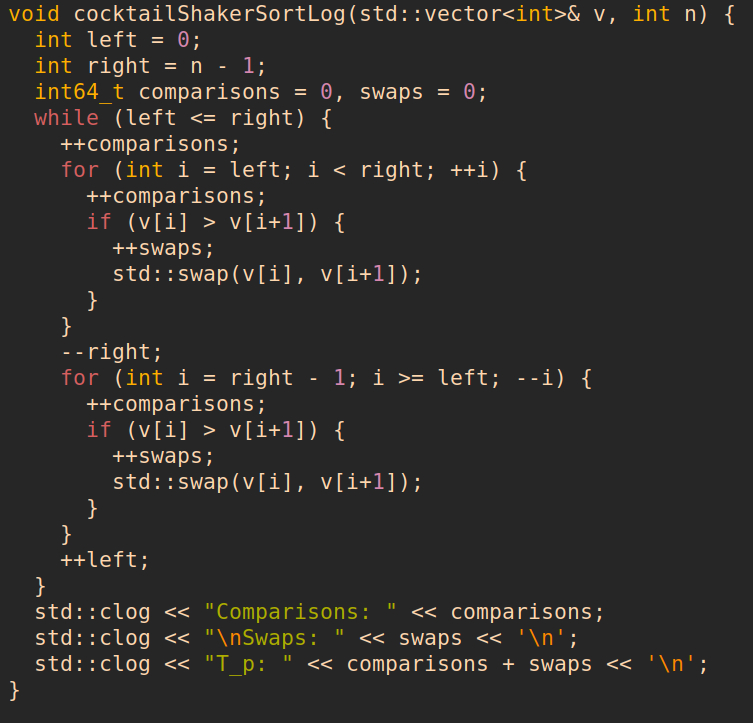
\includegraphics[width=0.7\textwidth]{pictures/second_sort_log.png}
  \caption{Функция cocktailShakerSortLog}
  \label{fig:second_sort_log}
\end{figure}

\newpage
\subsection{Анализ результатов 1-й и 2-й сортировок}
По таблицам \ref{tab:first_sort_test_general} и \ref{tab:second_sort_test_general}
непросто заметить разницу в скорости выполнения
сортировки. Несмотря на одинаковую асимптотическую сложность, шейкерная
сортировка все же в среднем имеет намного меньше операций перестановки по
сравнению с пузырьковой,
что можно заметить по практической вычислительной сложности алгоритма
и скорости выполнения программы.
Отсюда следует, что алгоритм шейкерной сортировки в
среднем случае эффективнее алгоритма сортировки пузырьком с условием
Айверсона.
\newpage
\subsection{Графики зависимостей практических вычислительных сложностей 1-й и 2-й сортировок}
\begin{figure}[htpb]
  \centering
  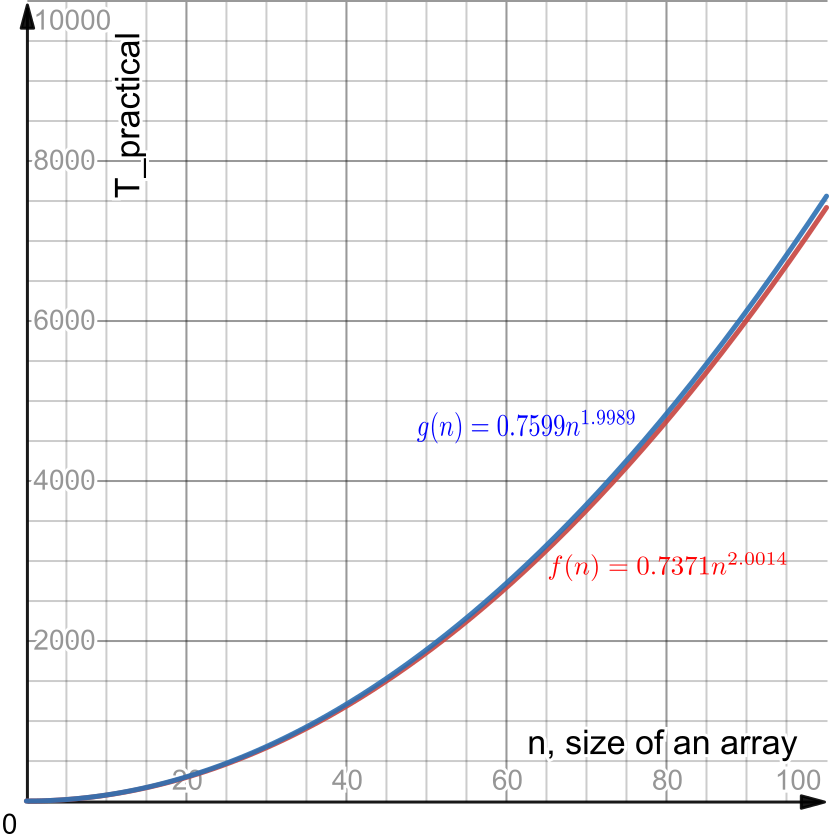
\includegraphics[width=0.7\textwidth]{pictures/first_comp_graph_test.png}
  \caption{Сравнение скоростей сортировок пузырьком и шейкерной}
  \label{fig:graph_first}
\end{figure}
На рис. \ref{fig:graph_first} приведены графики зависимостей практических
вычислительных сложностей алгоритмов сортировки пузырком с
условием Айверсона $f(n) = 0.7371n^{2.0014}$ и шейкерной сортировки от размера
n массива $g(n) = 0.7599n^{1.9989}$. По графикам можно заметить разницу в росте времени работы
алгоритмов – время работы шейкерной сортировки растет медленнее с
увеличением размера массива.
\newpage
\subsection{Сортировка слиянием}
\paragraph{Постановка задачи}
Разработать алгоритм сортировки простым слиянием.Сформировать
таблицу результатов для массива, заполненного случайными числами.
Определить емкостную сложность алгоритма. Определить асимптотическую
сложность алгоритма.
\paragraph{Описание алгоритма сортировки}
Сортировка слиянием состоит из двух главных действий:
\begin{enumerate}
  \item Разделить неотсортированный массив на $n$ подмассивов, каждый
    из которых содержит один элемент (т.е. массив считается отсортированным).
  \item Повторно производить слияние подмассивов для создания больших по
    размеру сортированных подмассивов, пока не останется единственный подмассив,
    который и будет нашим отсортированным массивом.
\end{enumerate}
\newpage
\paragraph{Алгоритм сортировки}
\begin{figure}[htpb]
  \centering
  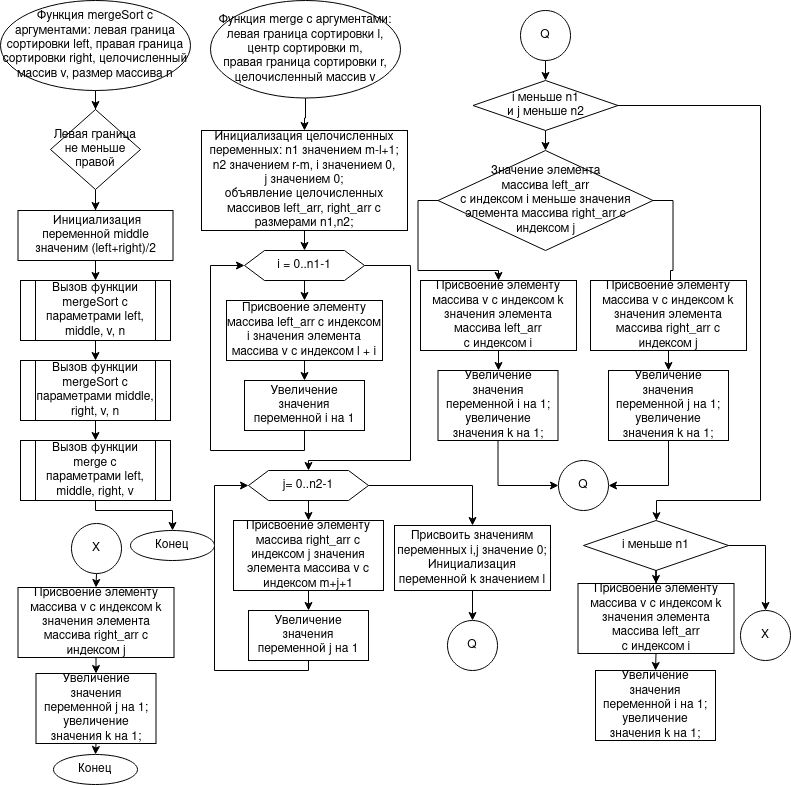
\includegraphics[width=0.9\textwidth]{pictures/third_sort_flowchart.png}
  \caption{Блок-схема сортировки простым слиянием}
  \label{fig:third_sort_flow}
\end{figure}

\paragraph{Оценка функции роста скорости выполнения алгоритма сортировки}
Временная сложность функции merge $ = \Theta(n)$ т.к. в функции нет вложенных
циклов и не происходят операции со скоростью меньше чем  $\Theta(n)$. 
Для оценки скорости выполнения рекурсивного алгоритма mergeSort сначала запишем
его в рекуррентом виде
\begin{equation}
T(n)=aT(\frac{n}{b})+f(n), \text{где } a\geq 1, b\geq 1
\end{equation}
где $n$ - размер задачи,  $a$ -  количество задач в подрекурсии,
$\frac{n}{b}$ - размер каждой подзадачи, $f(n)$ - оценка сложности работы,
производимой алгоритмом вне рекурсивных вызовов.
Для сортировки слиянием: $f(n) = \Theta(n)$, т.к. кроме рекурсивных вызовов происходят
только вызова функций со сложностью  $\Theta(n)$; $a = 2$ т.к. мы
вызываем две подзадачи; $b = 2$ т.к. мы разбиваем текущий массив на два подмассива.
Отсюда мы получаем \[
  T(n) = 2T(\frac{n}{2})+\Theta(n)
.\] 

По Мастер теореме: если $f(n) = \Theta(n)$, то тогда  $T(n) = \Theta(n\log n)$.
\paragraph{Емкостная сложность алгоритма}
Т.к. в данной задаче используются дополнительные массивы размера
входного массива $n$, то емкостная сложности алгоритма равняется $O(n)$
(также память расходуется на рекурсивные вызовы, но ими можно пренебречь
по сравнению с памятью на создание дополнительных массивов).
\newpage
\paragraph{Код функции сортировки}
\begin{figure}[htpb]
  \centering
  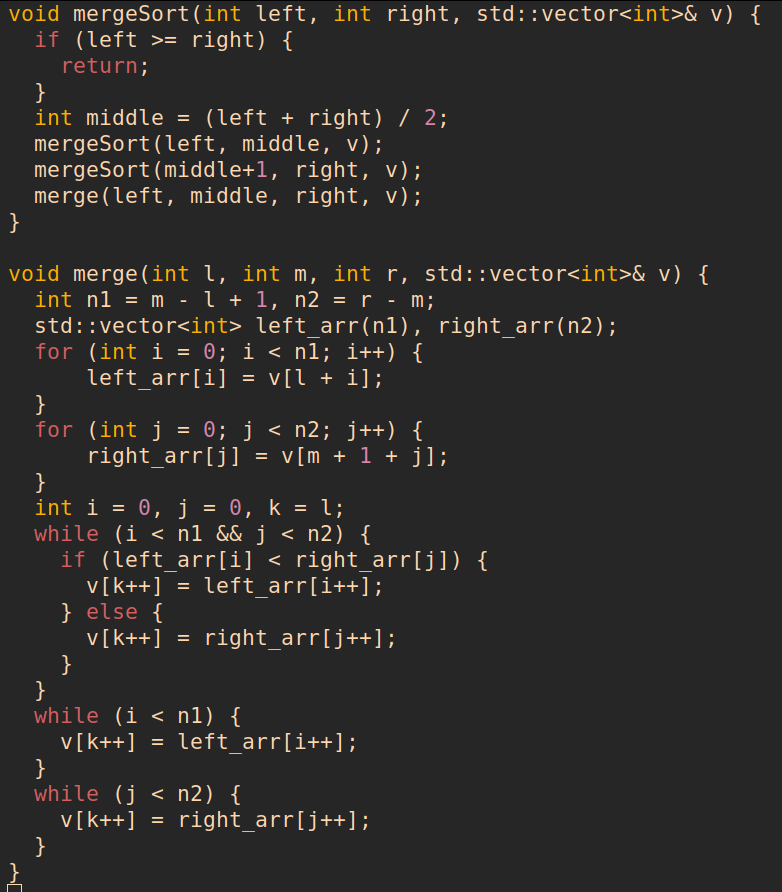
\includegraphics[width=0.7\textwidth]{pictures/third_sort_code.png}
  \caption{Код сортировки слиянием}
  \label{fig:first_sort_code}
\end{figure}
\newpage
\paragraph{Тестирование функции сортировки}
\begin{figure}[htpb]
  \centering
  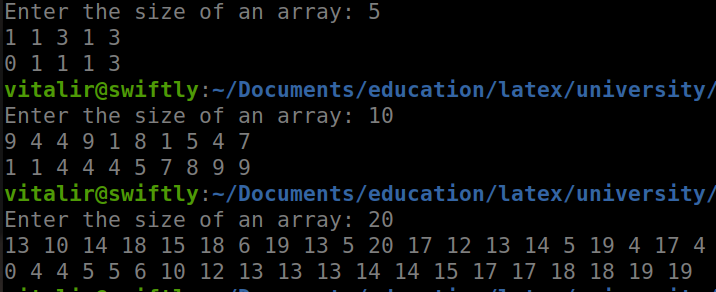
\includegraphics[width=0.6\textwidth]{pictures/third_sort_test.png}
  \caption{Результаты тестирования на работоспособность сортировки простым слиянием}
  \label{fig:first_sort_test}
\end{figure}
\paragraph{Сводная таблица тестирования}
\begin{figure}[htpb]
  \centering
  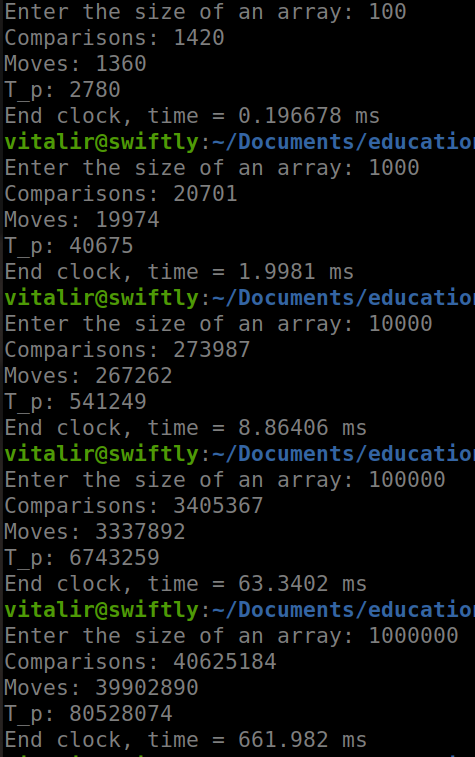
\includegraphics[scale=0.45]{pictures/third_sort_speed_gen.png}
  \caption{Результаты тестирования сортировки слиянием}
  \label{fig:third_sort_speed_gen}
\end{figure}
\newpage
\begin{table}[htpb]
  \centering
  \caption{Сводная таблица тестирования сортировки слиянием}
  \label{tab:third_sort_test_general}
  \begin{tabular}{|c|c|c|c|}
    \hline
    n & $T(n)$ & $T_\textup Т=f(C+M)$ &
    $T_\textup п=C_\textup ф+M_\textup ф$
    \\ \hline
    100
    & 0.196678 мс
    & \multirow{5}*{\centering $\Theta(n\log n)$}
    & 2780
    \\ \cline{1-2}\cline{4-4}
    1000
    & 1.9981 мс
    &
    & 40675
    \\ \cline{1-2}\cline{4-4}
    10000
    & 8.86406 мс
    &
    & 541249
    \\ \cline{1-2}\cline{4-4}
    100000
    & 63.3402 мс
    &
    & 6743259
    \\ \cline{1-2}\cline{4-4}
    1000000
    & 661.982 мс
    &
    & 80528074
    \\ \hline
  \end{tabular}
\end{table}
Для тестирования был использован класс для подсчета времени TimeCounter;
также была создана версия функции сортировки со встроенной отладкой.
(рисунки \ref{fig:time_counter_code} и \ref{fig:third_sort_log}).
\begin{figure}[htpb]
  \centering
  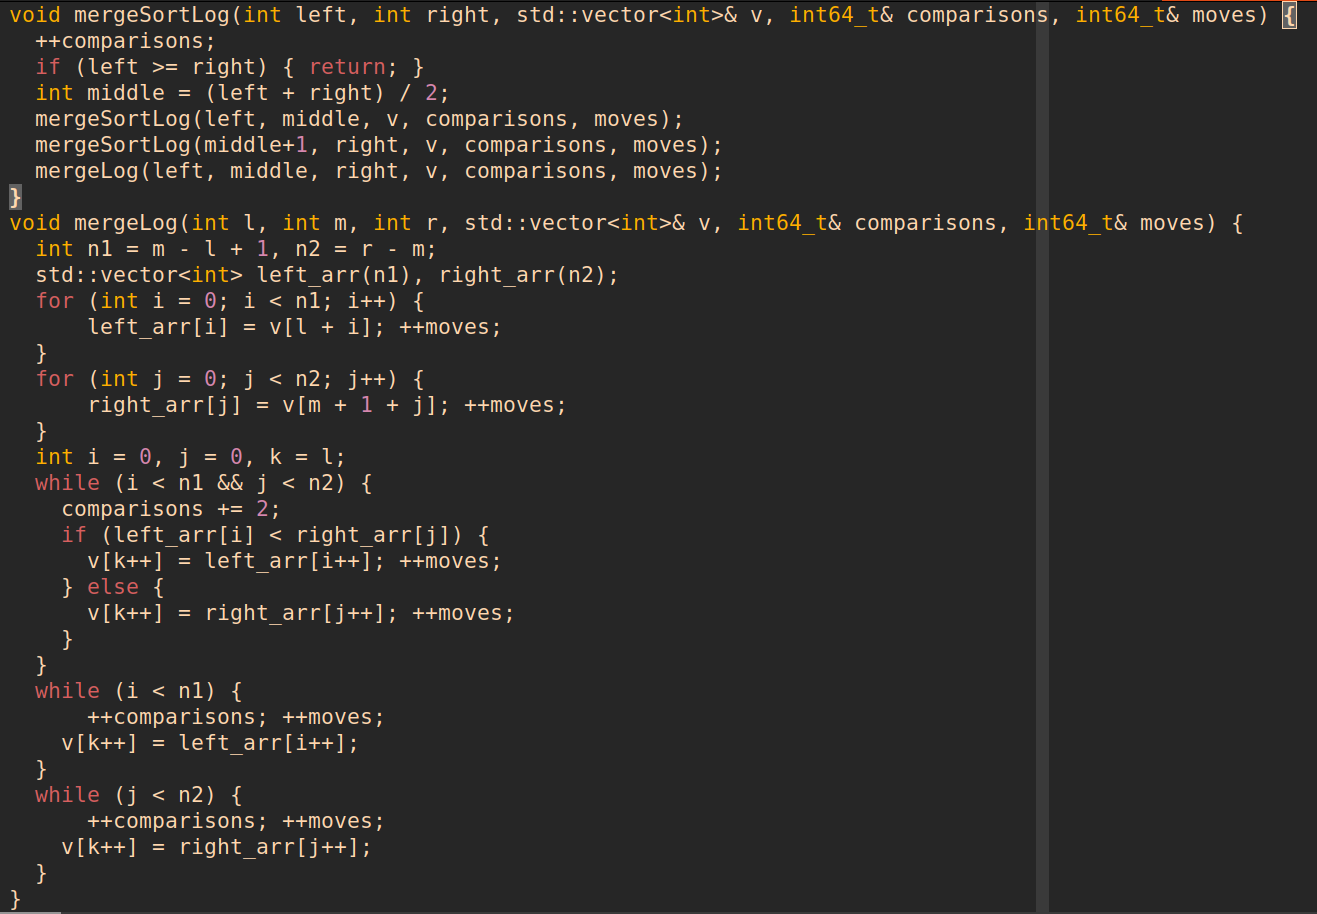
\includegraphics[width=0.9\textwidth]{pictures/third_sort_log.png}
  \caption{Функция mergeSortLog}
  \label{fig:third_sort_log}
\end{figure}


\subsection{Анализ результатов 2-й и 3-й сортировок}
Для сравнения шейкерной сортировки и сортировки простого слияния
сравним результаты из таблиц \ref{tab:second_sort_test_general} и
\ref{tab:third_sort_test_general}. Из таблиц
вычислительная сложность обоих алгоритмов повторяет найденную
теоретически, при этом сортировка слиянием с асимптотической сложностью
$\Theta(n\log n)$ превосходит в скорости работы шейкерную сортировку 
со сложностью $O(n^2)$.
Таким образом, алгоритм сортировки простым слиянием эффективнее
алгоритма шейкерной сортировки по временной
сложности в среднем случае.

\subsection{Графики зависимостей практических вычислительных сложностей 2-й и 3-й сортировок}
\begin{figure}[htpb]
  \centering
  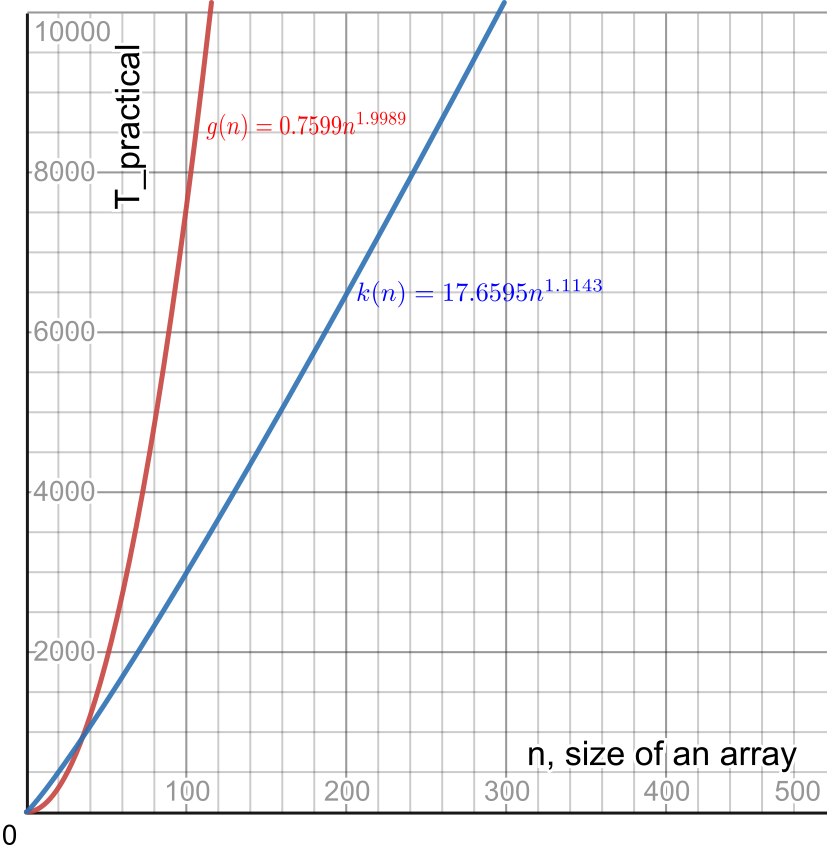
\includegraphics[width=0.8\textwidth]{pictures/second_comp_graph_tex.png}
  \caption{Сравнение скоростей шейкерной и простого слияния сортировок}
  \label{fig:graph_second}
\end{figure}
На рис. \ref{fig:graph_second} приведены графики зависимостей практических
вычислительных сложностей алгоритмов
шейкерной сортировки $g(n) = 0.7599n^{1.9989}$ и
сортировки слиянием $k(n) = 17.6595n^{1.1143}$.
По графикам можно заметить, что практическая сложность алгоритма сортировки
слиянием растет значительно медленней сложности шейкерной сортировки.
\newpage
\section{Задание 2. Определение эффективного из алгоритмов для наихудшего и
наилучшего случаев}
\subsection{Результаты тестирования алгоритмов на упорядоченных массивах}
\begin{figure}[htpb]
  \centering
  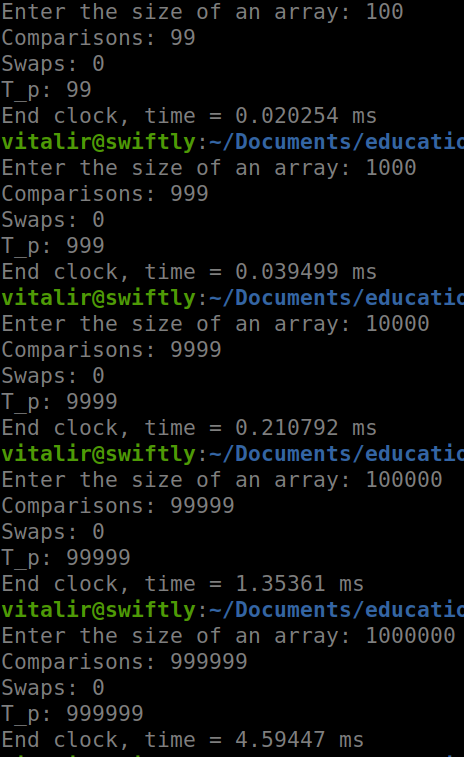
\includegraphics[width=0.45\textwidth]{pictures/first_sort_best.png}
  \caption{Результаты тестирования сортировки пузырьком с условием Айверсона в лучшем случае}
  \label{fig:first_sort_speed_best}
\end{figure}
\begin{table}[htpb]
  \centering
  \caption{Сводная таблица тестирования в лучшем случае}
  \label{tab:first_sort_test_best}
  \begin{tabular}{|c|c|c|c|}
    \hline
    n & $T(n)$ & $T_\textup Т=f(C+M)$ &
    $T_\textup п=C_\textup ф+M_\textup ф$
    \\ \hline
    100
    & 0.020254 мс
    & \multirow{5}*{\centering $O(n)$}
    & 99
    \\ \cline{1-2}\cline{4-4}
    1000
    & 0.039499 мс
    &
    & 999
    \\ \cline{1-2}\cline{4-4}
    10000
    & 0.210792 мс
    &
    & 9999
    \\ \cline{1-2}\cline{4-4}
    100000
    & 1.35361 мс
    &
    & 99999
    \\ \cline{1-2}\cline{4-4}
    1000000
    & 4.59447 мс
    &
    & 999999
    \\ \hline
  \end{tabular}
\end{table}
\newpage
\begin{figure}[htpb]
  \centering
  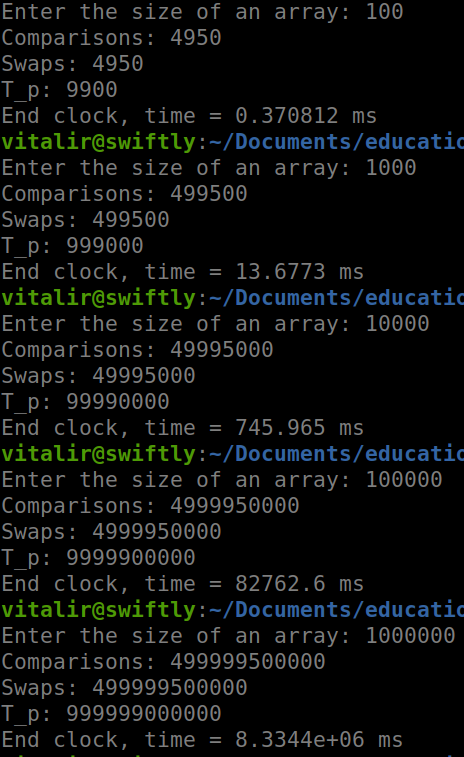
\includegraphics[width=0.45\textwidth]{pictures/first_sort_worst.png}
  \caption{Результаты тестирования сортировки пузырьком с условием Айверсона в худшем случае}
  \label{fig:first_sort_speed_worst}
\end{figure}
\begin{table}[htpb]
  \centering
  \caption{Сводная таблица тестирования в худшем случае}
  \label{tab:first_sort_test_worst}
  \begin{tabular}{|c|c|c|c|}
    \hline
    n & $T(n)$ & $T_\textup Т=f(C+M)$ &
    $T_\textup п=C_\textup ф+M_\textup ф$
    \\ \hline
    100
    & 0.370012 мс
    & \multirow{5}*{\centering $O(n^2)$}
    & 9900
    \\ \cline{1-2}\cline{4-4}
    1000
    & 13.6673 мс
    &
    & 999000
    \\ \cline{1-2}\cline{4-4}
    10000
    & 745.965 мс
    &
    & 99990000
    \\ \cline{1-2}\cline{4-4}
    100000
    & 82762.6 мс
    &
    & 9999900000
    \\ \cline{1-2}\cline{4-4}
    1000000
    & 833440 мс
    &
    & 999999000000
    \\ \hline
  \end{tabular}
\end{table}
\newpage
\begin{figure}[htpb]
  \centering
  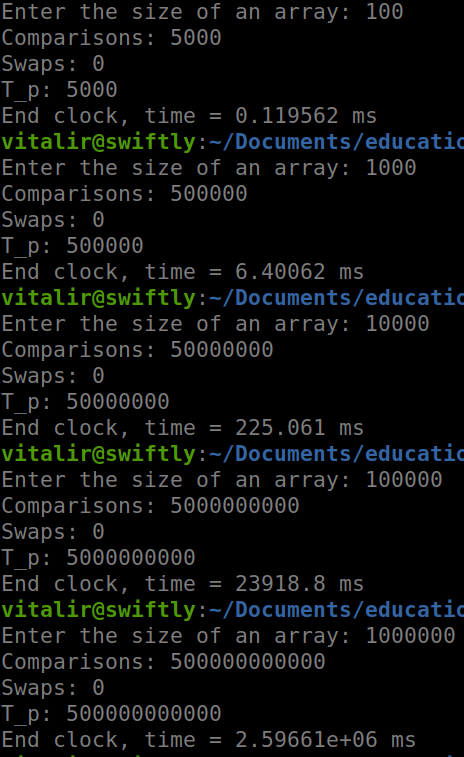
\includegraphics[width=0.45\textwidth]{pictures/second_sort_best.png}
  \caption{Результаты тестирования шейкерной сортировки в лучшем случае}
  \label{fig:second_sort_speed_best}
\end{figure}
\begin{table}[htpb]
  \centering
  \caption{Сводная таблица тестирования в лучшем случае}
  \label{tab:second_sort_test_best}
  \begin{tabular}{|c|c|c|c|}
    \hline
    n & $T(n)$ & $T_\textup Т=f(C+M)$ &
    $T_\textup п=C_\textup ф+M_\textup ф$
    \\ \hline
    100
    & 0.119562 мс
    & \multirow{5}*{\centering $O(n^2)$}
    & 5000
    \\ \cline{1-2}\cline{4-4}
    1000
    & 6.40062 мс
    &
    & 500000
    \\ \cline{1-2}\cline{4-4}
    10000
    & 225.061 мс
    &
    & 50000000
    \\ \cline{1-2}\cline{4-4}
    100000
    & 23918.8 мс
    &
    & 5000000000
    \\ \cline{1-2}\cline{4-4}
    1000000
    & 2596610 мс
    &
    & 500000000000
    \\ \hline
  \end{tabular}
\end{table}
\newpage
\begin{figure}[htpb]
  \centering
  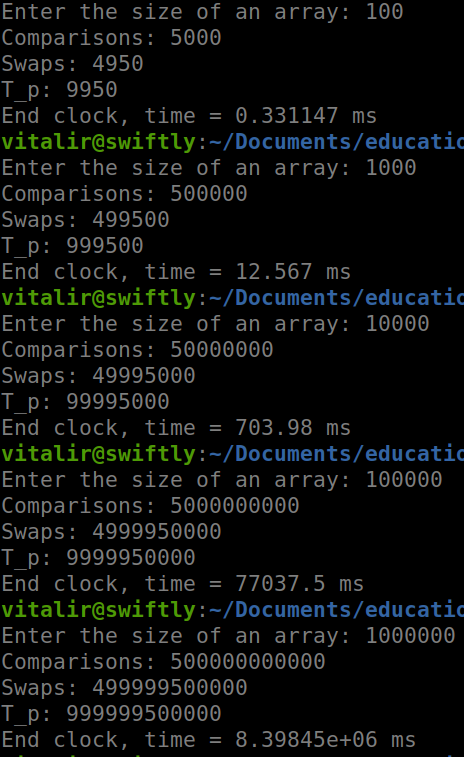
\includegraphics[width=0.45\textwidth]{pictures/second_sort_worst.png}
  \caption{Результаты тестирования шейкерной сортировки в худшем случае}
  \label{fig:second_sort_speed_worst}
\end{figure}
\begin{table}[htpb]
  \centering
  \caption{Сводная таблица тестирования в худшем случае}
  \label{tab:second_sort_test_worst}
  \begin{tabular}{|c|c|c|c|}
    \hline
    n & $T(n)$ & $T_\textup Т=f(C+M)$ &
    $T_\textup п=C_\textup ф+M_\textup ф$
    \\ \hline
    100
    & 0.331147 мс
    & \multirow{5}*{\centering $O(n^2)$}
    & 9950
    \\ \cline{1-2}\cline{4-4}
    1000
    & 12.567 мс
    &
    & 999500
    \\ \cline{1-2}\cline{4-4}
    10000
    & 703.98 мс
    &
    & 99995000
    \\ \cline{1-2}\cline{4-4}
    100000
    & 77037.5 мс
    &
    & 9999950000
    \\ \cline{1-2}\cline{4-4}
    1000000
    & 8398450 мс
    &
    & 999999500000
    \\ \hline
  \end{tabular}
\end{table}
\newpage
\begin{figure}[htpb]
  \centering
  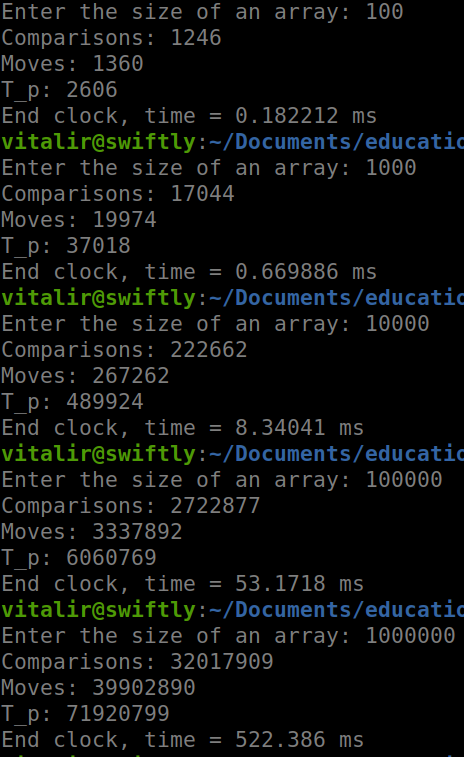
\includegraphics[width=0.45\textwidth]{pictures/third_sort_best.png}
  \caption{Результаты тестирования сортировки слиянием в лучшем случае}
  \label{fig:third_sort_speed_best}
\end{figure}
\begin{table}[htpb]
  \centering
  \caption{Сводная таблица тестирования в лучшем случае}
  \label{tab:third_sort_test_best}
  \begin{tabular}{|c|c|c|c|}
    \hline
    n & $T(n)$ & $T_\textup Т=f(C+M)$ &
    $T_\textup п=C_\textup ф+M_\textup ф$
    \\ \hline
    100
    & 0.182212 мс
    & \multirow{5}*{\centering $\Theta(n\log n)$}
    & 2606
    \\ \cline{1-2}\cline{4-4}
    1000
    & 0.669886 мс
    &
    & 37018
    \\ \cline{1-2}\cline{4-4}
    10000
    & 8.34041 мс
    &
    & 489924
    \\ \cline{1-2}\cline{4-4}
    100000
    & 53.1718 мс
    &
    & 6060769
    \\ \cline{1-2}\cline{4-4}
    1000000
    & 522.386 мс
    &
    & 71920799
    \\ \hline
  \end{tabular}
\end{table}
\newpage
\begin{figure}[htpb]
  \centering
  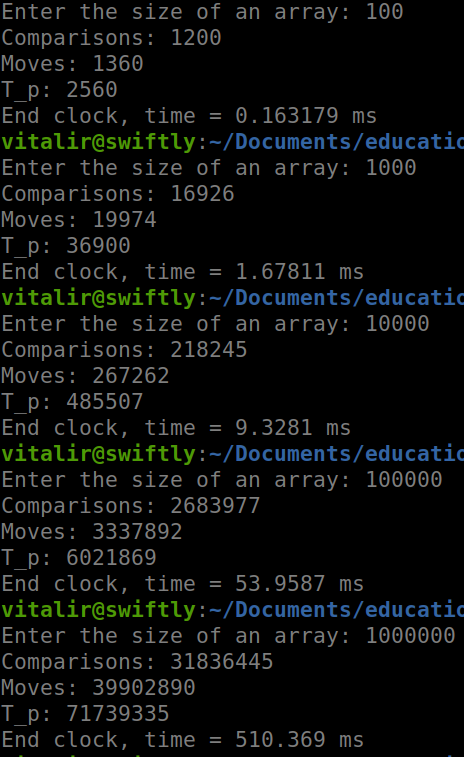
\includegraphics[width=0.45\textwidth]{pictures/third_sort_worst.png}
  \caption{Результаты тестирования сортировки слиянием в худшем случае}
  \label{fig:third_sort_speed_worst}
\end{figure}
\begin{table}[htpb]
  \centering
  \caption{Сводная таблица тестирования в худшем случае}
  \label{tab:third_sort_test_worst}
  \begin{tabular}{|c|c|c|c|}
    \hline
    n & $T(n)$ & $T_\textup Т=f(C+M)$ &
    $T_\textup п=C_\textup ф+M_\textup ф$
    \\ \hline
    100
    & 0.163179 мс
    & \multirow{5}*{\centering $\Theta(n\log n)$}
    & 2560
    \\ \cline{1-2}\cline{4-4}
    1000
    & 1.67811 мс
    &
    & 36900
    \\ \cline{1-2}\cline{4-4}
    10000
    & 9.3281 мс
    &
    & 485507
    \\ \cline{1-2}\cline{4-4}
    100000
    & 53.9587 мс
    &
    & 6021869
    \\ \cline{1-2}\cline{4-4}
    1000000
    & 510.369 мс
    &
    & 71739335
    \\ \hline
  \end{tabular}
\end{table}

\begin{figure}[htpb]
  \centering
  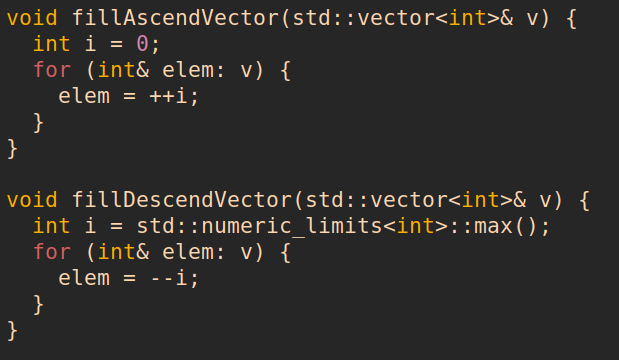
\includegraphics[width=0.7\textwidth]{pictures/code_order_arrays.png}
  \caption{Код функций для заполнения массивов по возрастанию и убыванию}
  \label{fig:test_sort_code_bw}
\end{figure}
Функции для тестирования сортировки в лучшем и худшем случаях представлены на рисунке
\ref{fig:test_sort_code_bw}.

\subsection{Асимптотическая сложность алгоритмов в лучшем и худшем случаях}
Алгоритм сортировки пузырьком с условием Айверсона: в лучшем случае
имеет асимптотическую сложность $O(n)$, в худшем -  $O(n^2)$.

Алгоритм шейкерной сортировки: в лучшем и худшем случаях имеет асимптотическую
сложность $O(n^2)$.

Алгоритм сортировки слиянием: в лучшем и худшем случаях имеет асимптотическую
сложность $\Theta(n\log n)$.

Из вышерасмотренных алгоритмов самым эффективным является алгоритм сортировки
слиянием, имея значительное преимущество во временной асимптотической сложности.

\subsection{Таблица асимптотической сложности алгоритмов}
\begin{table}[htpb]
  \centering
  \caption{Асимптотическая сложность алгоритмов, рассмотренных в данной работе}
  \label{tab:all_algs}
  \begin{tabular}{|c|c|c|c|c|}
    \hline
    \multirow{3}*{Алгоритм} & \multicolumn{4}{|c|}{Асимптотическая сложность алгоритма}
    \\ \hline
                            & \multirow{2}*{\parbox[m]{2.5cm}{\centering Наихудший\\ случай}}
                            & \multirow{2}*{\parbox[m]{2.5cm}{\centering Наилучший\\ случай}}
    & \multirow{2}*{\parbox[m]{2.5cm}{\centering Средний \\ случай}}
    & \multirow{2}*{\parbox[m]{4cm}{\centering Емкостная \\ сложность}}
 \\ & & & &
    \\ \hline
    \parbox[m]{2.5cm}{\centering Сортировка пузырьком с условием Айверсона}
    & $O(n)$ &  $O(n^2)$ & $O(n^2)$ & $O(n)$
    \\ \hline
    \parbox[m]{2.5cm}{\centering Шейкерная сортировка}
    & $O(n^2)$ &  $O(n^2)$ & $O(n^2)$ & $O(n)$
    \\ \hline
    \parbox[m]{2.5cm}{\centering Сортировка простым слиянием}
    & $\Theta(n\log n)$ & $\Theta(n\log n)$ & $\Theta(n\log n)$
    & \parbox[m]{4cm}{\centering $O(n)$,\\  $O(n)$ дополнительно}
    \\ \hline
  \end{tabular}
\end{table}


\section*{Выводы}
\addcontentsline{toc}{section}{Выводы}
В ходе практической работы были разработаны алгоритмы сортировки
простого обмена с условием Айверсона, шейкерной сортировки
и сортировки простого слияния, приобретены навыки по анализу
вычислительной сложности алгоритмов сортировки и определен наиболее
эффективный алгоритм (сортировка простым слиянием).
\section*{Список используемой литературы}
\addcontentsline{toc}{section}{Список используемой литературы}
\begin{enumerate}[leftmargin=*] % delete left margin
  \item Thomas H. Cormen, Clifford Stein и другие: Introduction to Algorithms, 3rd Edition.
    Сентябрь 2009. The MIT Press.
  \item B. Strousrup: A Tour of C++ (2nd Edition). Июль 2018. Addison-Wesley.
  \item Merge sort~//~Wikipedia \\~
    [Электронный ресурс]. URL:
    \\ https://en.wikipedia.org/wiki/Merge\_sort 
    (Дата обращения: 18.04.2021)
   \item Курс Algorithms, part 1 // Coursera [Электронный ресурс]. URL:
     \\ https://www.coursera.org/learn/algorithms-part1
     (Дата обращения: 18.04.2021)
\end{enumerate}
\end{document}
